\section{Resultados con features transformadas}
\label{sec:resultados_features_transformadas}

La Sección~\ref{sec:resultados_features_original} presentó los resultados del $\Delta$AIC 
para las features en escala original. En esta sección se evalúa el efecto 
de aplicar transformaciones sobre dichas features, con el objetivo de 
determinar si una representación alternativa mejora su capacidad predictiva 
sobre la señal EEG. 

\subsection{Diagnóstico de multicolinealidad (VIF)}

Al igual que para las features en escala original, se calculó el VIF 
para cada feature transformada incorporándola individualmente al modelo 
base MD2. La Tabla~\ref{tab:vif_features_transformadas} reporta la 
media, la mediana y el porcentaje de sujetos con VIF superior a 3 y 
a 5 para cada feature transformada.

\begin{table}[H]
\centering
\small
\begin{tabular}{lcccc}
\toprule
\textbf{Feature} & \textbf{Media} & \textbf{Mediana} & \textbf{\% sujetos VIF $>$ 3} & \textbf{\% sujetos VIF $>$ 5} \\
\midrule
\multicolumn{5}{l}{\textit{Bottom-up}} \\
\feat{saliencia\_pixel\_log}        & 2.83 & 2.78 & 11.9 & 0.0 \\
\feat{saliencia\_media\_log}        & 3.09 & 3.08 & 54.8 & 0.0 \\
\midrule
\multicolumn{5}{l}{\textit{Similitud con el target}} \\
\feat{similitud\_pixel\_log}        & 2.85 & 2.85 & 4.8  & 0.0 \\
\feat{similitud\_media\_log}        & 3.67 & 3.65 & 100.0 & 0.0 \\
\midrule
\multicolumn{5}{l}{\textit{Estado interno del proceso bayesiano}} \\
\feat{ganancia\_informacion\_log}   & 4.46 & 4.50 & 100.0 & 7.1 \\
\feat{posterior\_log}               & 10.50 & 10.47 & 100.0 & 100.0 \\
\feat{posterior\_logit}             & 9.88 & 9.91 & 100.0 & 100.0 \\
\midrule
\multicolumn{5}{l}{\textit{Calidad de la decisión}} \\
\feat{gap\_entropia\_log}           & 1.43 & 1.43 & 0.0  & 0.0 \\
\feat{distancia\_grilla\_log}       & 5.69 & 5.63 & 100.0 & 92.9 \\
\midrule
\multicolumn{5}{l}{\textit{Competencia entre candidatos}} \\
\feat{competencia\_densidad\_log}   & 6.36 & 6.49 & 100.0 & 100.0 \\
\feat{competencia\_fp\_max\_log}    & 1.48 & 1.48 & 0.0  & 0.0 \\
\bottomrule
\end{tabular}
\caption{VIF calculado por sujeto para cada feature transformada, 
incorporada individualmente al modelo base MD2. Se reportan la 
media y mediana grupal ($n = 42$) y el porcentaje de sujetos que 
superan los umbrales de VIF $>$ 3 y VIF $>$ 5.}
\label{tab:vif_features_transformadas}
\end{table}

Se puede observar en la tabla cómo algunas de las transformaciones introducen multicolinealidad problemática 
con los predictores del modelo base. Las transformaciones 
\feat{posterior\_log} y \feat{posterior\_logit} presentaron los 
valores más elevados, con medias de 10.50 y 9.88 respectivamente 
y el 100\% de los sujetos superando el umbral de VIF $> 5$. 
\feat{competencia\_densidad\_log} y \feat{distancia\_grilla\_log} 
también superaron dicho umbral, con medias de 6.36 y 5.69 y el 
100\% y 92.9\% de los sujetos afectados respectivamente. Estas 
cuatro features fueron descartadas del análisis de $\Delta$AIC 
y TFCE correspondiente.

Las 7 features transformadas restantes presentaron valores de VIF 
aceptables.


\subsection{Evaluación individual de features mediante $\Delta$ AIC}

Para cada feature, se compara el $\Delta$AIC obtenido 
al incorporar la versión transformada al modelo base MD2 contra el 
$\Delta$AIC correspondiente a la versión en escala original. En la mayoría de los casos la transformación 
$\log(x)$ mejora el ajuste respecto a la versión base, con la 
excepción de \feat{gap\_entropia\_log}.

\begin{figure}[H]
    \centering
    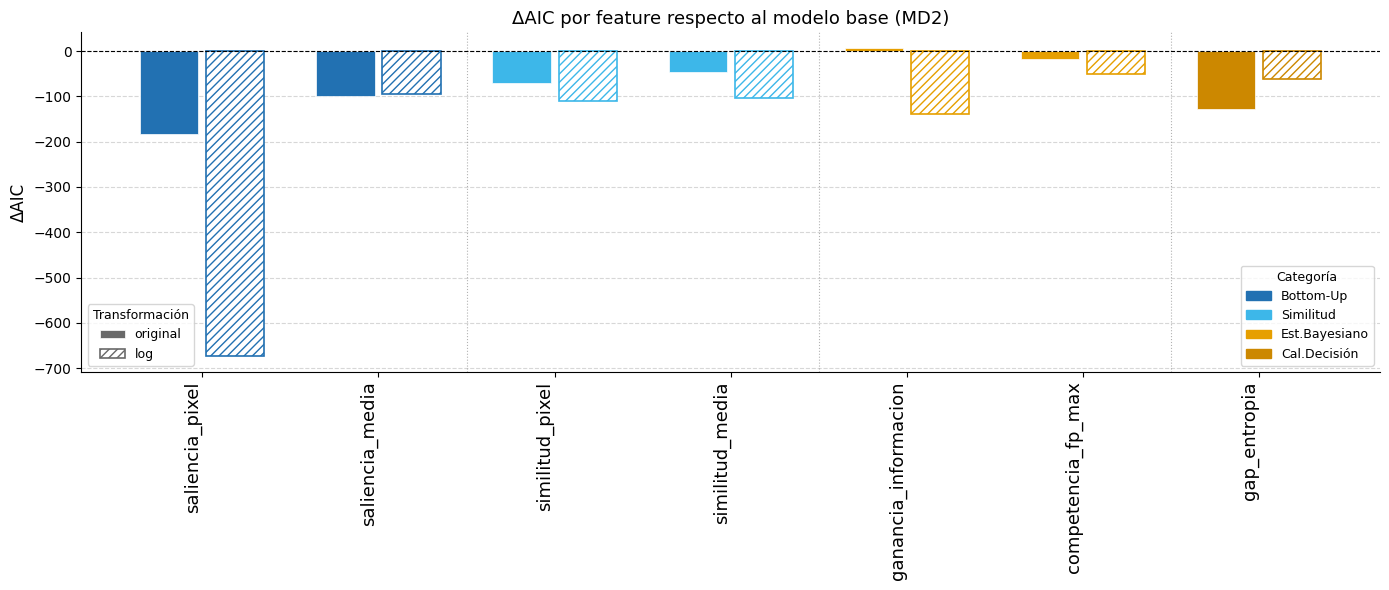
\includegraphics[width=\textwidth]{chapters/04_resultados/images/delta_aic_transformadas}
    \caption{$\Delta$AIC para features en escala original y transformadas, coloreadas por categoría}
    \label{fig:delta_aic_transformadas}
\end{figure}

La feature \feat{saliencia\_pixel\_log} presenta 
la mayor ganancia de todo el conjunto evaluado ($\Delta$AIC $= 
-673{,}97$ vs. $-182{,}97$ en escala original), consolidándose 
como la feature con mayor capacidad predictiva sobre la señal EEG. 
En contraste, \feat{saliencia\_media\_log} no muestra una mejora 
apreciable respecto a su versión original ($\Delta$AIC $= -94{,}59$ 
vs. $-99{,}20$), sugiriendo que la transformación logarítmica no 
aporta información adicional para esta feature.

En la categoría de similitud con el target, tanto 
\feat{similitud\_pixel\_log} ($\Delta$AIC $= -110{,}11$ vs. 
$-70{,}15$) como \feat{similitud\_media\_log} ($\Delta$AIC $= 
-103{,}08$ vs. $-45{,}29$) muestran mejoras moderadas respecto 
a sus versiones originales.

En el caso de \feat{ganancia\_informacion}, la transformación produce el cambio más pronunciado: mientras que en escala original su $\Delta$AIC era positivo ($7{,}43$), la transformación 
$\log(x)$ revierte este comportamiento de forma marcada, resultando 
en $\Delta$AIC $= -138{,}17$. Este resultado sugiere que la 
relación entre \feat{ganancia\_informacion} y la señal EEG es 
esencialmente no lineal en escala original, y que la transformación 
logarítmica captura esta relación de forma más adecuada.

En la categoría de competencia entre candidatos, 
\feat{competencia\_fp\_max\_log} muestra una mejora moderada 
respecto a su versión original ($\Delta$AIC $= -50{,}63$ vs. 
$-18{,}45$).

Finalmente, \feat{gap\_entropia\_log} es el único caso en que 
la transformación empeora el ajuste respecto a la versión original 
($\Delta$AIC $= -62{,}56$ vs. $-127{,}46$), lo que indica que 
la escala original captura mejor la relación de esta feature con 
la señal EEG.

\subsection{Resultados TFCE: Significancia Estadística Espacio-Temporal}

La significancia estadística de los efectos fue evaluada mediante TFCE 
para las 7 features transformadas que superaron el diagnóstico de multicolinealidad.
Para cada feature, los resultados se comparan con 
los obtenidos en su versión en escala original, con el objetivo de 
determinar si la transformación modifica no solo la magnitud del 
$\Delta$AIC sino también la presencia y extensión de clusters 
espacio-temporales significativos. Los resultados se organizan en 
tres grupos: features con clusters significativos en ambas versiones, 
features que obtienen clusters significativos únicamente en la versión 
transformada, y features sin clusters significativos en ninguna de las 
dos versiones.

\subsubsection{Features con clusters significativos en ambas versiones}

Las features \feat{saliencia\_pixel}, \feat{saliencia\_media} y 
\feat{similitud\_pixel} presentaron clusters significativos tanto en 
su versión en escala original como en su versión transformada, aunque 
con diferencias en la extensión espacio-temporal de los clusters.

\pendiente{Análisis de FRPs (componentes, amplitud, consistencia, etc.)}

\begin{figure}[H]
    \centering
    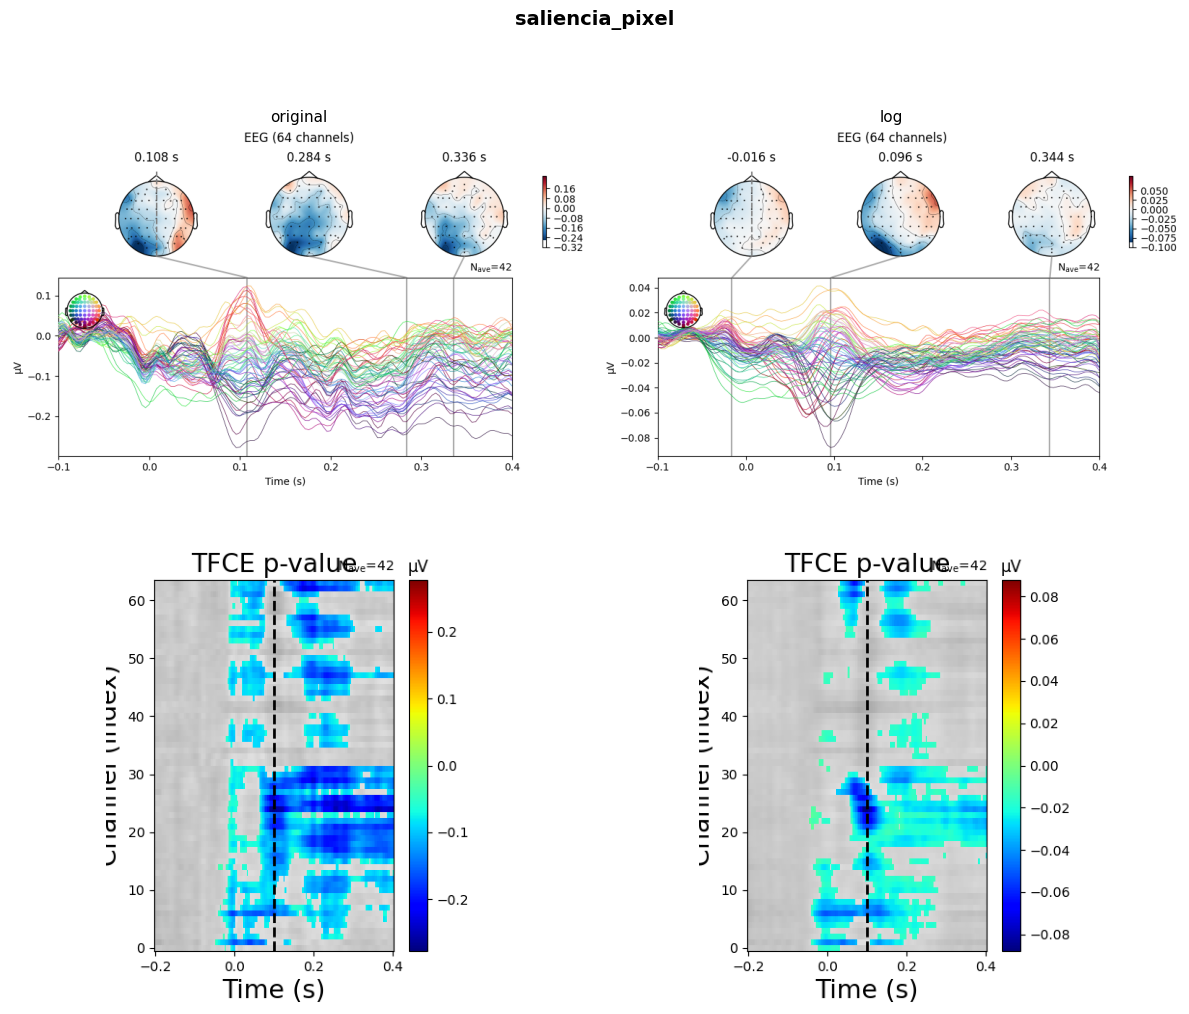
\includegraphics[width=0.7\textwidth]{chapters/04_resultados/images/TFCE_saliencia_pixel.png}
    \caption{Comparación resultados de TFCE para \feat{saliencia\_pixel} original y transformada en escala logarítmica.}
    \label{fig:tfce_saliencia_pixel}
\end{figure}

\begin{figure}[H]
    \centering
    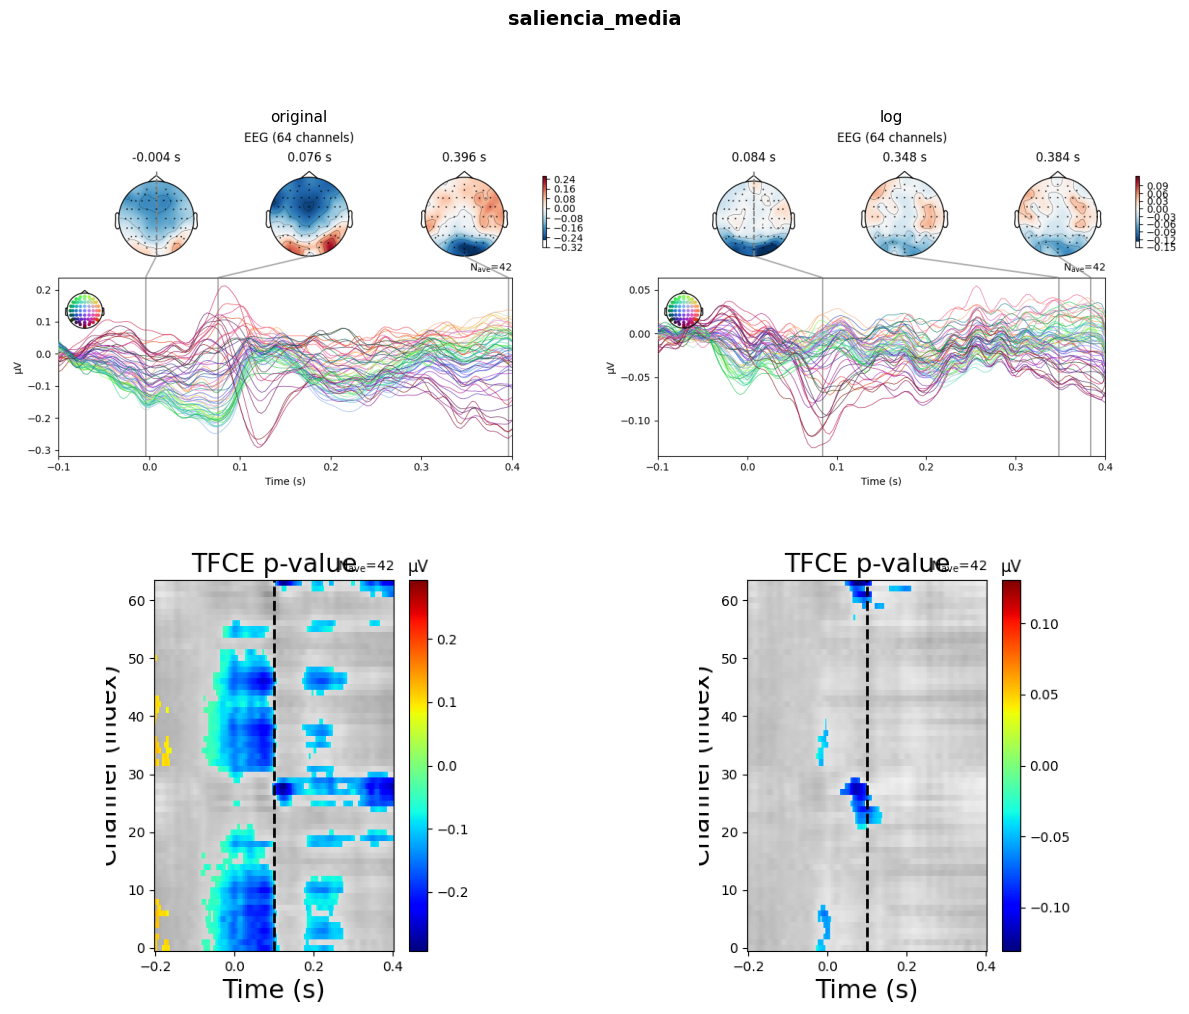
\includegraphics[width=0.7\textwidth]{chapters/04_resultados/images/TFCE_saliencia_media.png}
    \caption{Comparación resultados de TFCE para \feat{saliencia\_media} original y transformada en escala logarítmica.}
    \label{fig:tfce_saliencia_media}
\end{figure}

\begin{figure}[H]
    \centering
    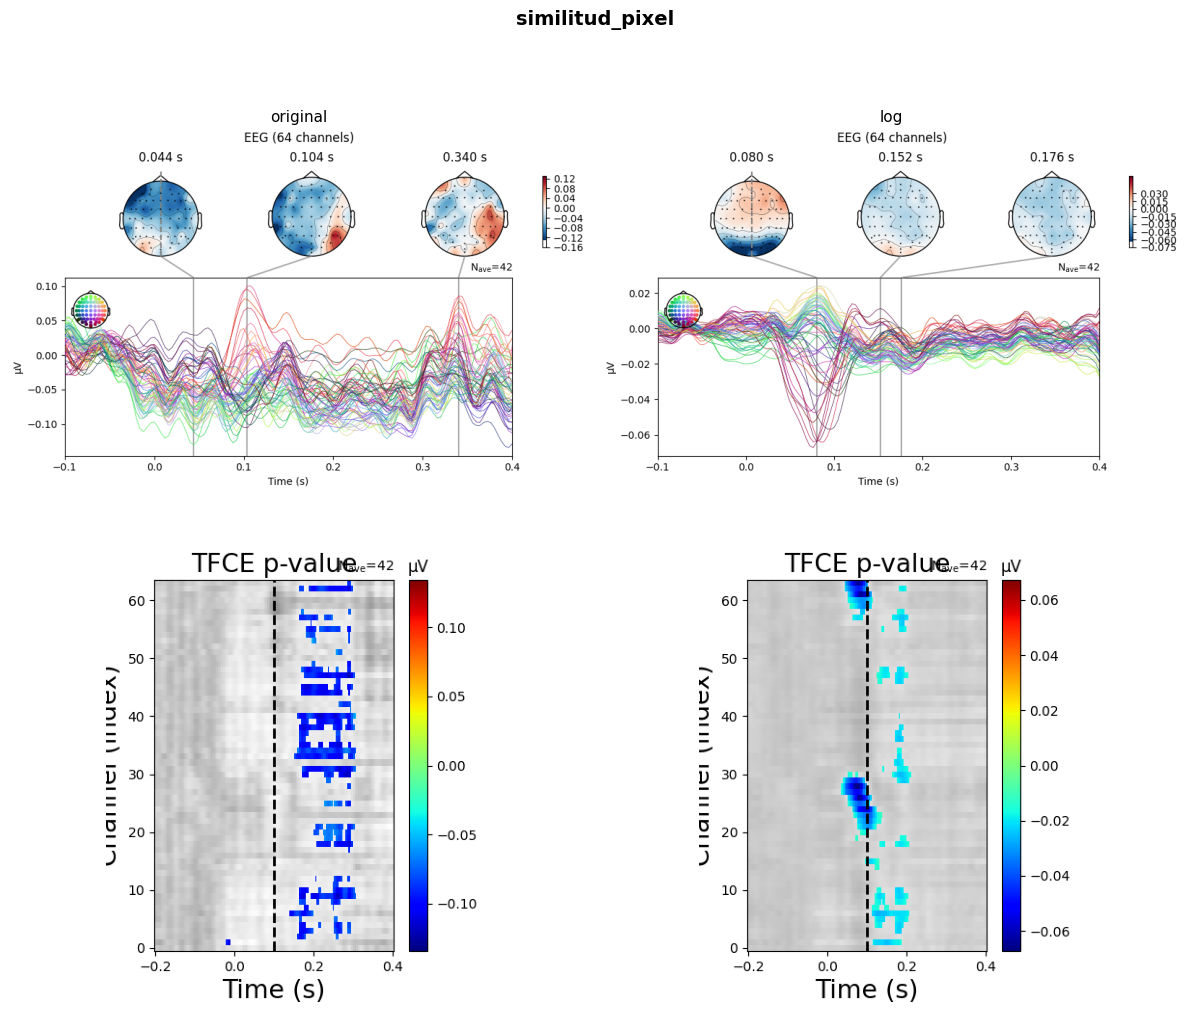
\includegraphics[width=0.7\textwidth]{chapters/04_resultados/images/TFCE_similitud_pixel.png}
    \caption{Comparación resultados de TFCE para \feat{saliencia\_media} original y transformada en escala logarítmica.}
    \label{fig:tfce_similitud_pixel}
\end{figure}

\subsubsection{Features con clusters significativos solo en la versión transformada}

Las features \feat{similitud\_media}, \feat{ganancia\_informacion} y 
\feat{gap\_entropia} no presentaron clusters significativos en escala 
original pero sí en su versión transformada, lo que indica que la 
transformación logarítmica permite detectar efectos que no eran 
evidentes en la escala original.

\pendiente{Análisis de FRPs (componentes, amplitud, consistencia, etc.)}

\begin{figure}[H]
    \centering
    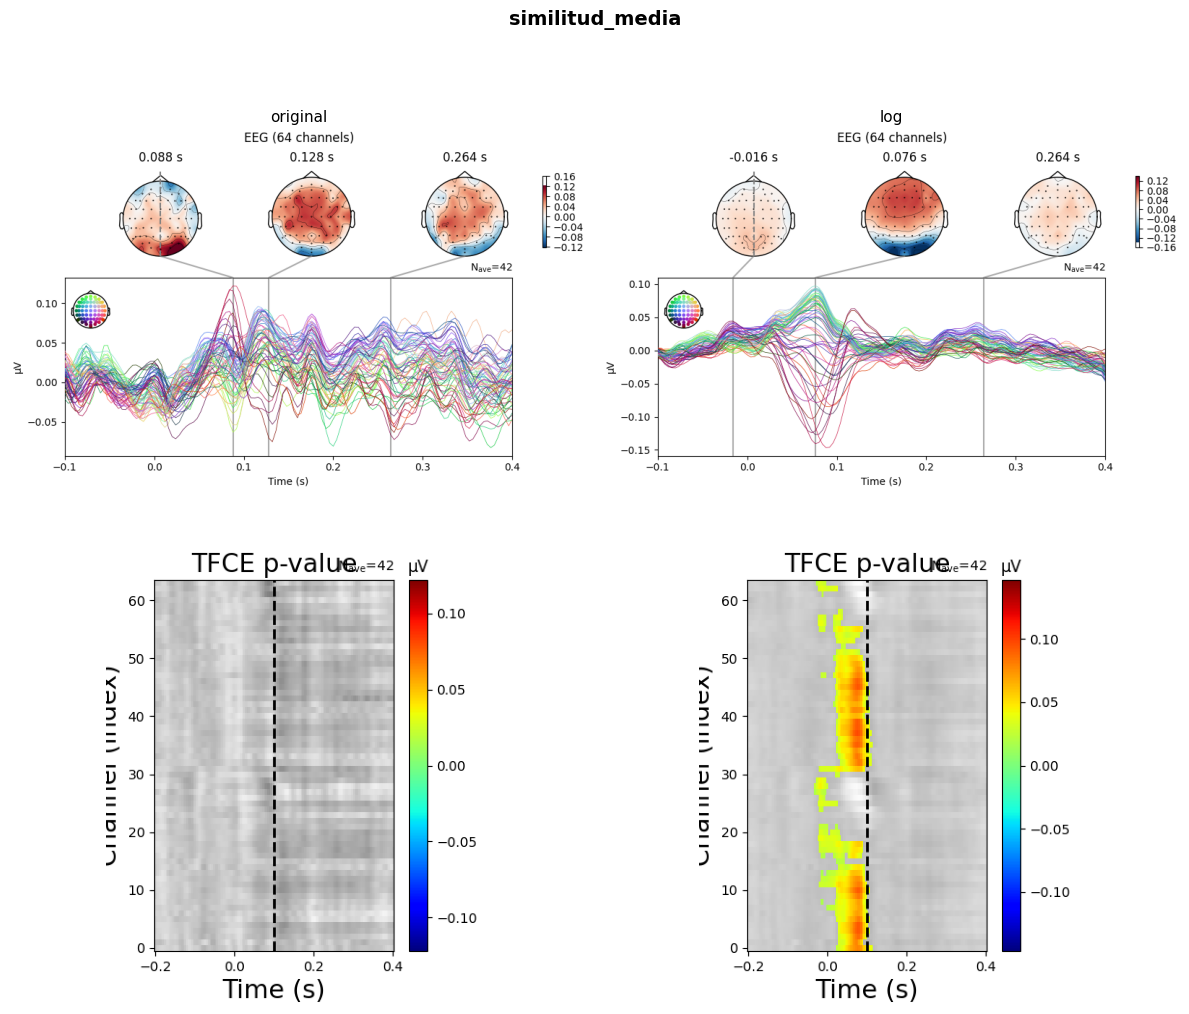
\includegraphics[width=0.7\textwidth]{chapters/04_resultados/images/TFCE_similitud_media.png}
    \caption{Comparación resultados de TFCE para \feat{similitud\_media} original y transformada en escala logarítmica.}
    \label{fig:tfce_similitud_media}
\end{figure}

\begin{figure}[H]
    \centering
    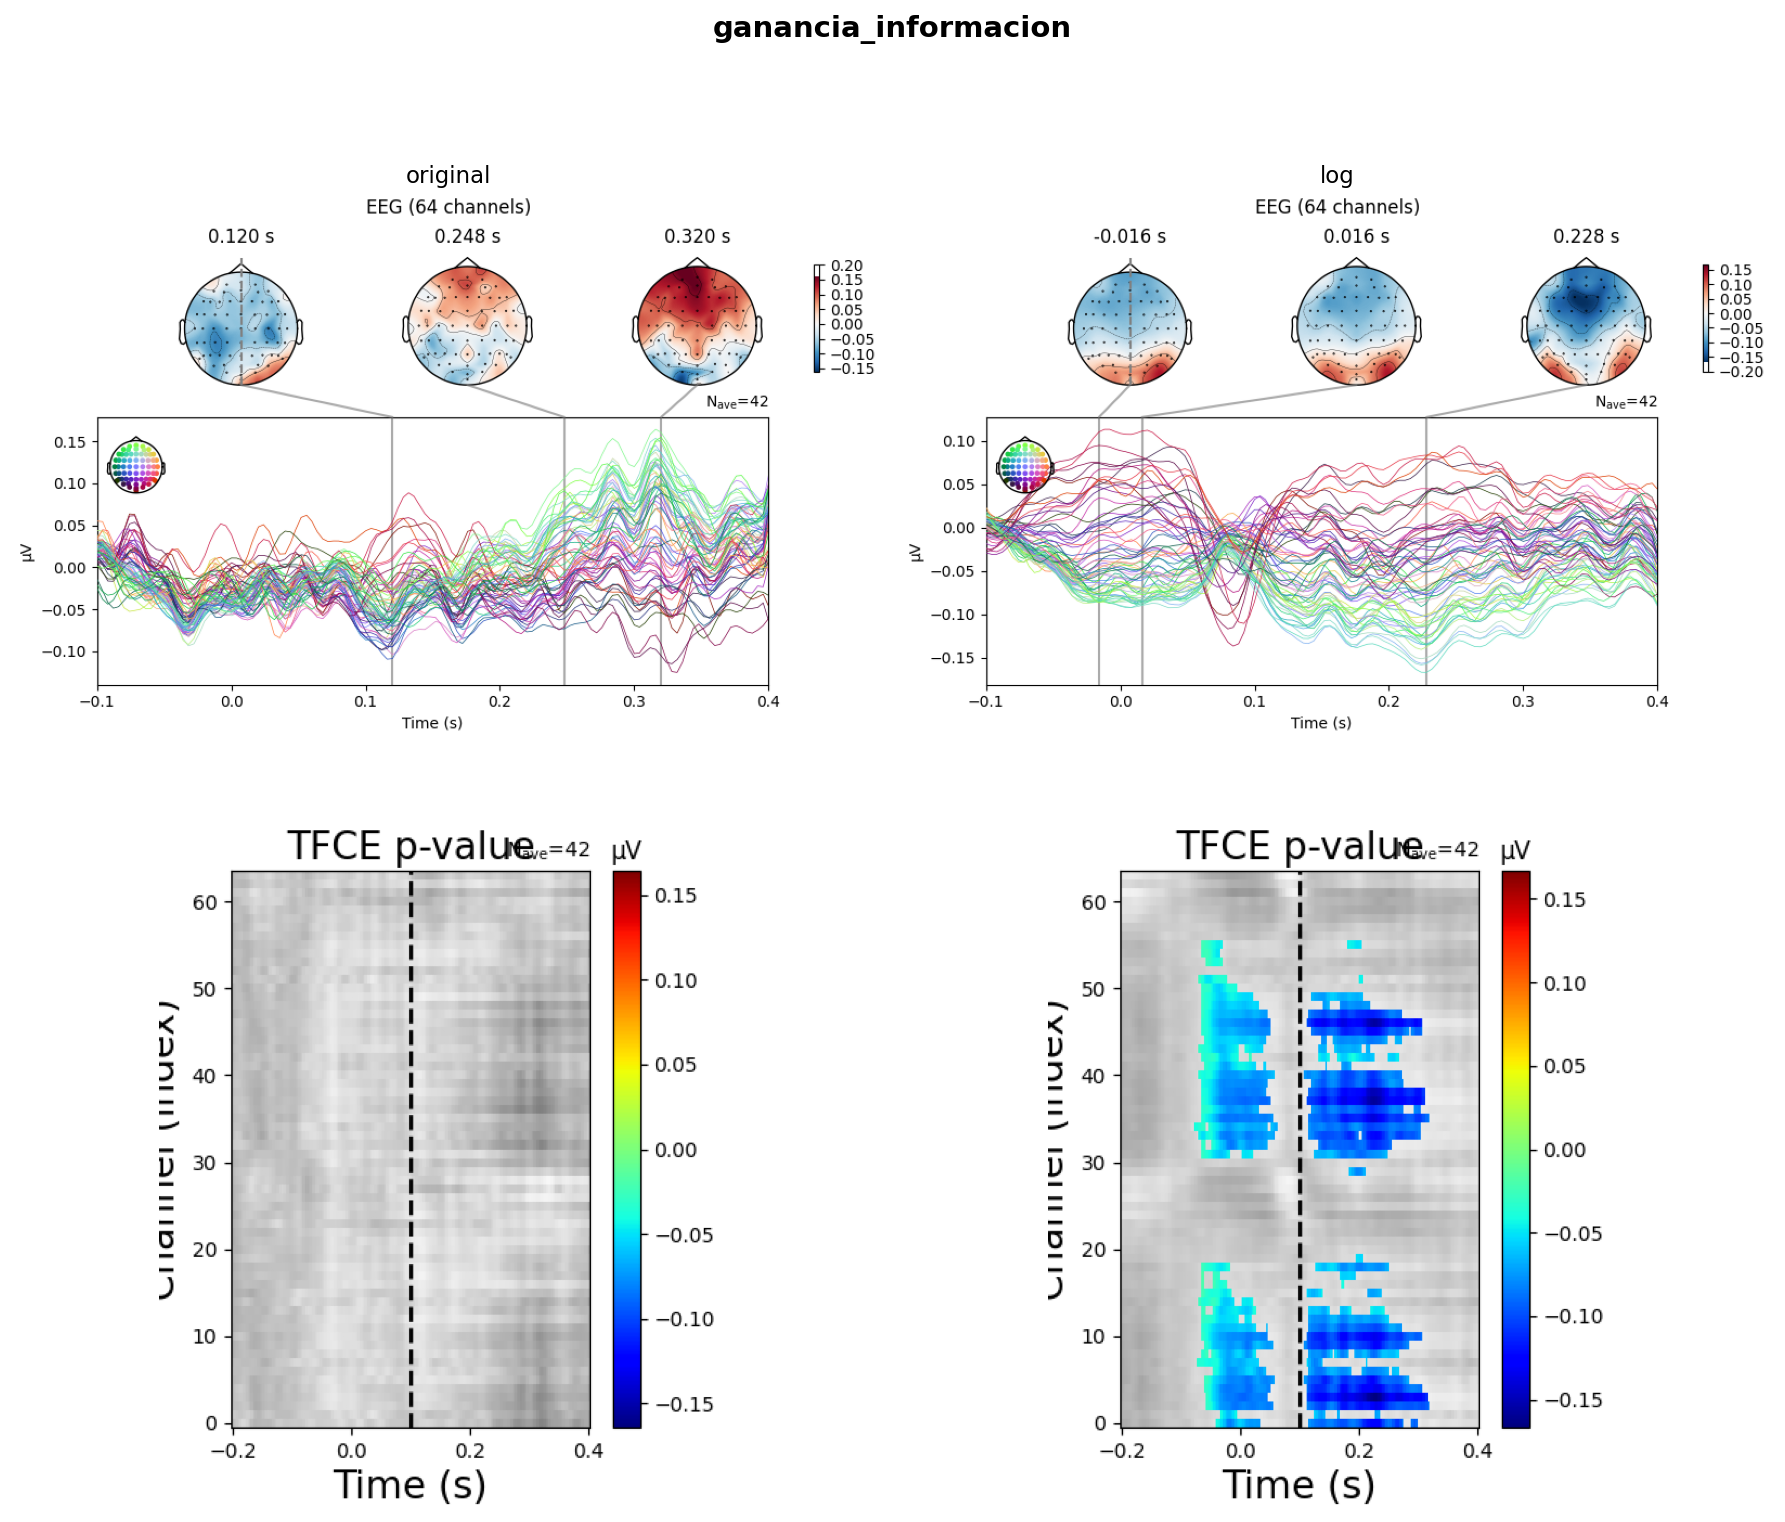
\includegraphics[width=0.7\textwidth]{chapters/04_resultados/images/TFCE_ganancia_informacion.png}
    \caption{Comparación resultados de TFCE para \feat{ganancia\_informacion} original y transformada en escala logarítmica.}
    \label{fig:tfce_ganancia_informacion}
\end{figure}

\begin{figure}[H]
    \centering
    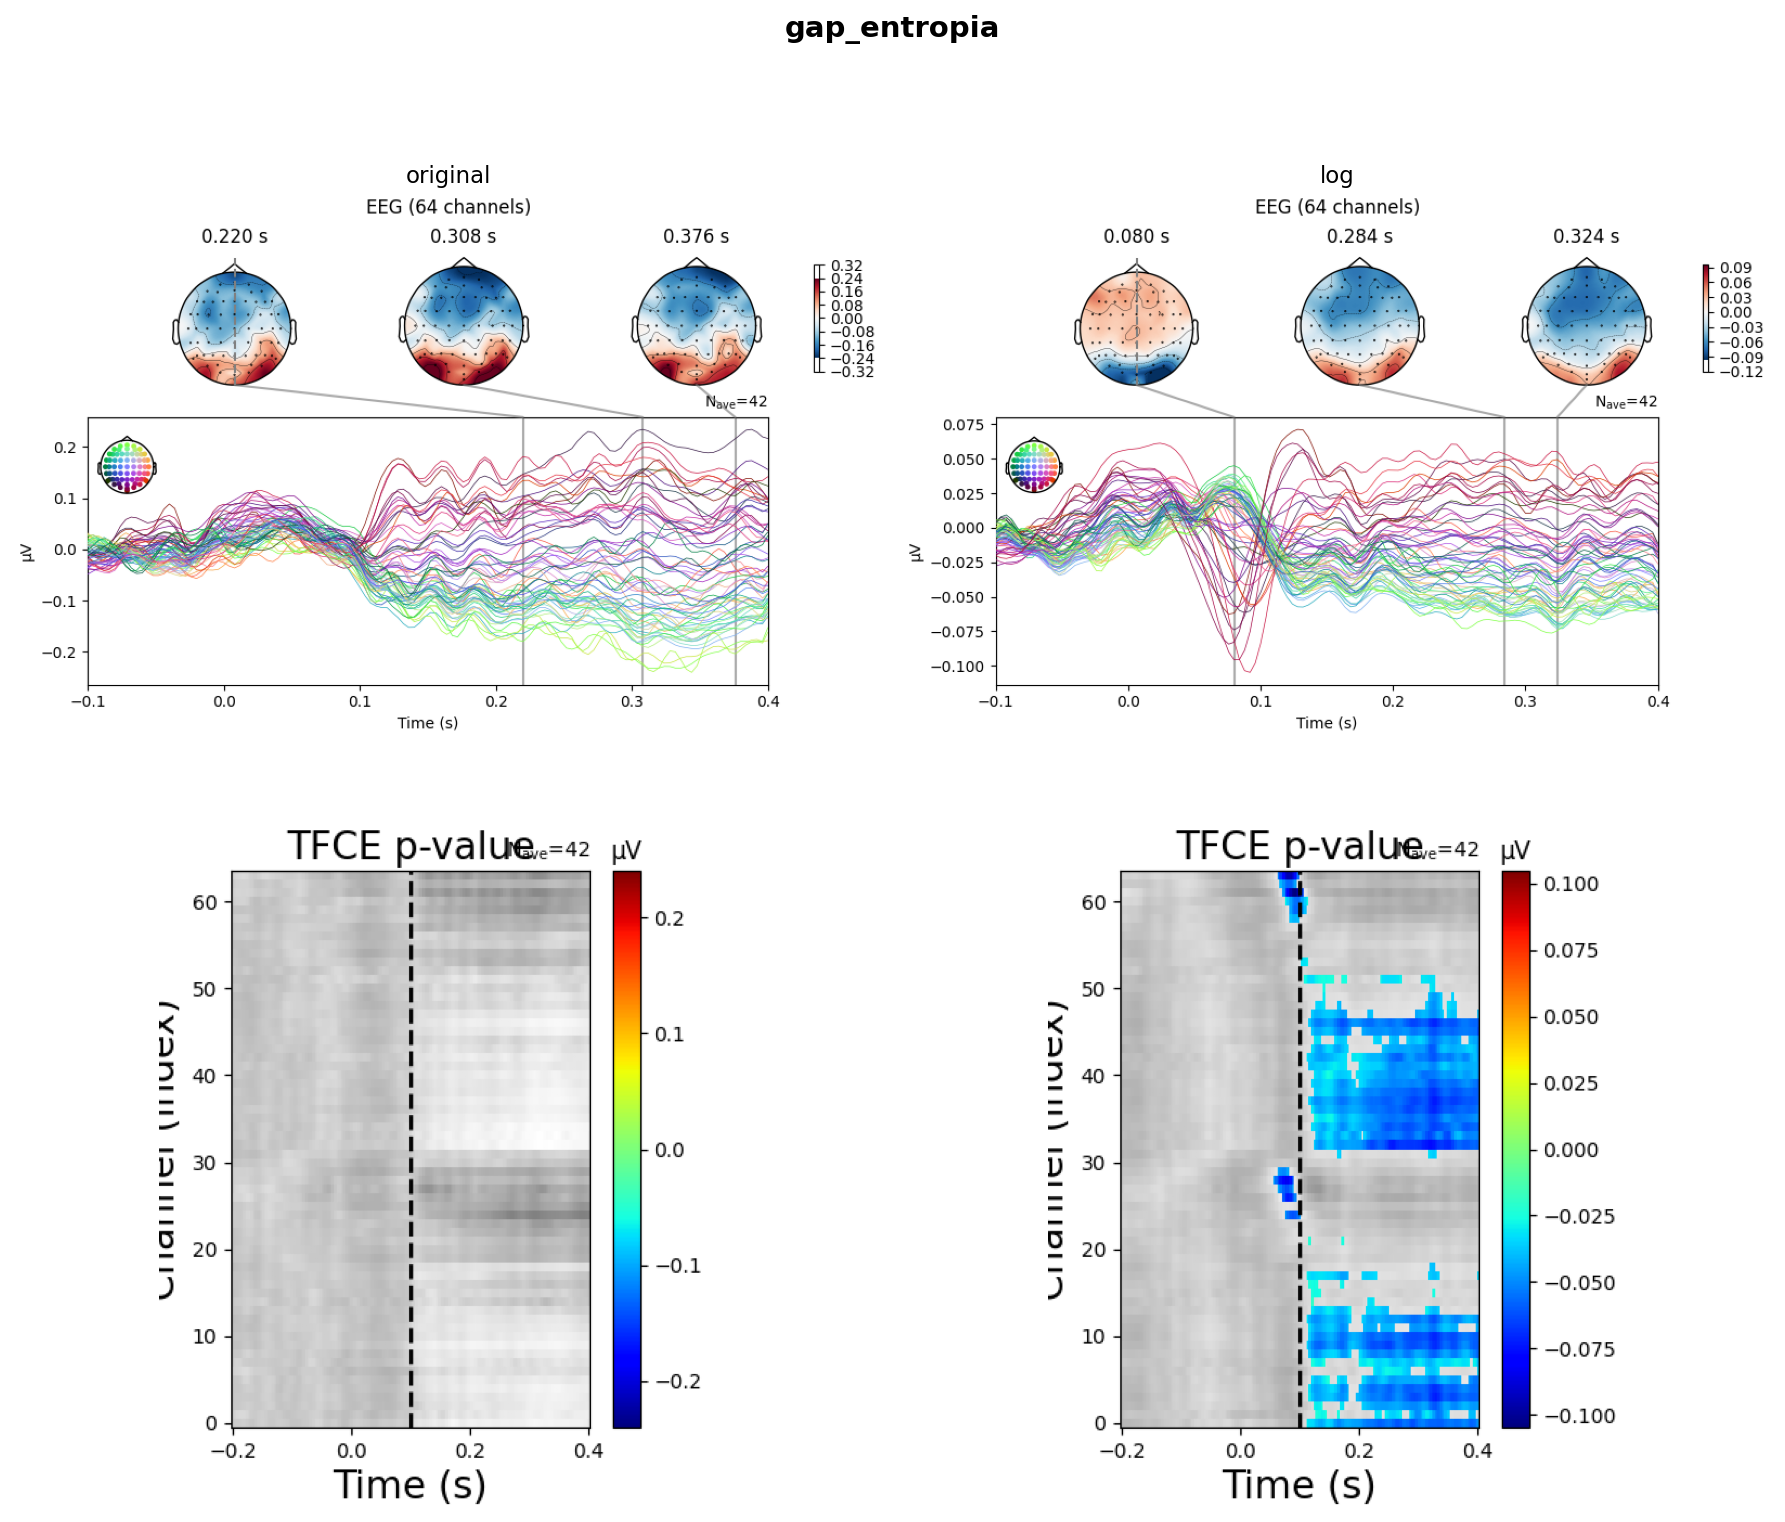
\includegraphics[width=0.7\textwidth]{chapters/04_resultados/images/TFCE_gap_entropia.png}
    \caption{Comparación resultados de TFCE para \feat{gap\_entropia} original y transformada en escala logarítmica.}
    \label{fig:tfce_gap_entropia}
\end{figure}


\subsubsection{Features sin clusters significativos en ninguna versión}

\feat{competencia\_fp\_max} y \feat{competencia\_fp\_max\_log} no 
presentaron clusters espacio-temporales significativos según el criterio 
TFCE en ninguna de las dos versiones. Este resultado es consistente 
con los valores moderados de $\Delta$AIC observados para ambas versiones: si bien la transformación 
logarítmica mejora el ajuste del modelo respecto al baseline, esta 
mejora no se traduce en efectos estadísticamente significativos a nivel 
espacio-temporal.

\begin{figure}[H]
    \centering
    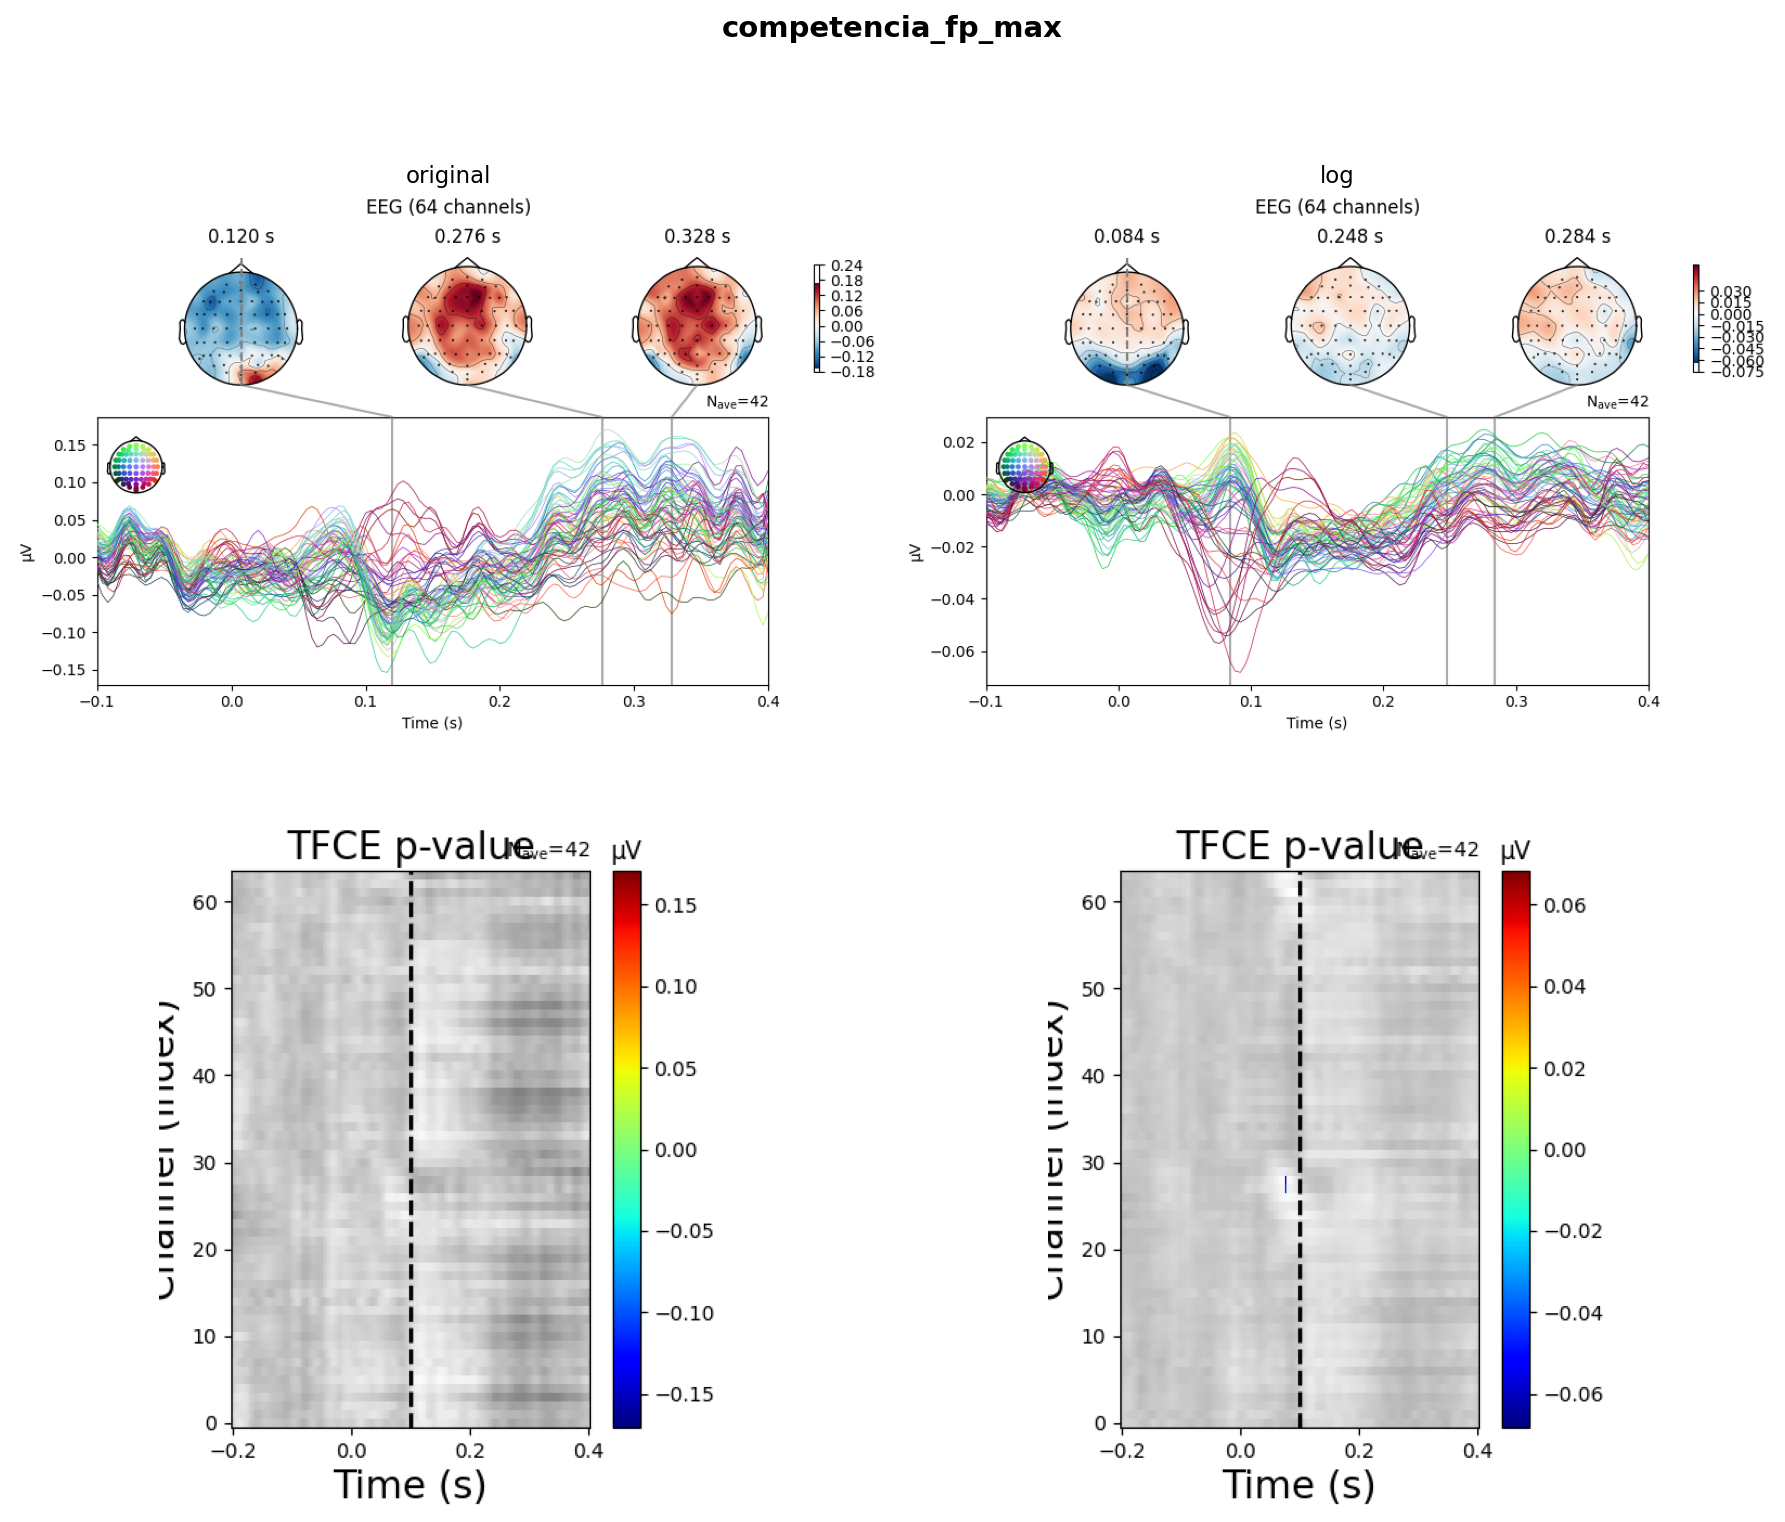
\includegraphics[width=0.7\textwidth]{chapters/04_resultados/images/TFCE_competencia_fp_max.png}
    \caption{Comparación resultados de TFCE para \feat{competencia\_fp\_max} original y transformada en escala logarítmica.}
    \label{fig:tfce_competencia_fp_max}
\end{figure}
